\documentclass[12pt]{article}

% -------------------- preamble --------------------
\usepackage{amsthm}
\newtheorem*{exercise}{Exercise}
\newtheorem*{solution}{Solution}
\usepackage{amsmath, amssymb}
\usepackage{physics}
\usepackage{geometry}
\usepackage{hyperref}
\usepackage{nicematrix}
\usepackage{empheq}
\usepackage{xcolor}
\usepackage{tikz}
\usetikzlibrary{positioning}

\newcommand*\widefbox[1]{\fbox{\hspace{2em}#1\hspace{2em}}}

\geometry{margin=1in}

\title{Lecture Notes: Tensors for Beginners\\
\large Based on Youtube series by eigenchris}
\author{}
\date{}

% -------------------- document --------------------
\begin{document}
\maketitle
\tableofcontents
\newpage

% -------------------- input sections --------------------
\section{Motivation: Coordinate Independence in Physics}

Physical laws must not depend on how we label space.

\subsection*{Why Does This Matter?}

In physics, we describe phenomena using mathematical equations. However, these equations should describe reality itself, not our particular choice of coordinates. Consider:

\begin{itemize}
    \item \textbf{Newton's Laws}: The force on an object doesn't change if you rotate your coordinate system
    \item \textbf{Maxwell's Equations}: Electromagnetic fields behave the same regardless of your reference frame
    \item \textbf{General Relativity}: The curvature of spacetime is independent of coordinate choice
\end{itemize}

This principle is fundamental: \emph{physical reality is invariant, even though our descriptions of it may change with coordinates}.

\subsection*{Example: Velocity}
A particle moving in space has a velocity that exists independently of coordinates.
If we rotate our coordinate axes, the particle does not suddenly move differently — only the \emph{numbers} describing its velocity change.

For instance, a ball moving northward at 5 m/s has the same physical motion whether you describe it in:
\begin{itemize}
    \item Coordinates aligned north-south and east-west
    \item Coordinates rotated 45 degrees
    \item Polar coordinates centered at your location
\end{itemize}

The velocity vector itself (the geometric object) remains the same. Only its components (the numbers in your coordinate system) change.

\subsection*{The Core Distinction}

This distinction between:
\begin{itemize}
    \item the geometric object (velocity)
    \item its coordinate representation (components)
\end{itemize}
is the core motivation for tensors.

\subsection*{Key Principle}
\begin{quote}
If a quantity represents something physical or geometric, then changing coordinates must not change the object itself, only how we describe it.
\end{quote}

Tensors are defined so this principle is automatically satisfied. They provide a mathematical framework where:
\begin{enumerate}
    \item Objects exist independently of coordinates
    \item We can compute how their components transform when we change coordinates
    \item Physical laws written in tensor notation are automatically coordinate-independent
\end{enumerate}

\subsection*{Thought Exercises}

\begin{exercise}
Consider the following physical quantities. For each, identify whether it is coordinate-independent (invariant) or coordinate-dependent:
\begin{enumerate}
    \item The temperature at a point in space
    \item The velocity components $(v_x, v_y, v_z)$ of a moving particle
    \item The speed (magnitude of velocity) of a moving particle
    \item The coordinates $(x, y, z)$ of a point in space
    \item The distance between two points
    \item Newton's second law: $\vec{F} = m\vec{a}$
\end{enumerate}
\textit{Hint: Ask yourself, "If I rotate my coordinate system, does this quantity change?"}
\end{exercise}

\begin{exercise}
Understanding the distinction:
\begin{enumerate}
    \item A car travels east at 60 km/h. You set up coordinates with the x-axis pointing north. What are the velocity components in your coordinate system?
    \item Your friend uses coordinates with the x-axis pointing east. What are the velocity components in their coordinate system?
    \item Did the car's motion change between parts (a) and (b)? What changed?
    \item Explain why we need a mathematical framework that distinguishes between "the velocity" and "the velocity components"
\end{enumerate}
\end{exercise}

\begin{exercise}
Why tensors matter in physics:
\begin{enumerate}
    \item If Maxwell's equations were not coordinate-independent, what would this imply about electromagnetic phenomena?
    \item In general relativity, gravity is described by the curvature of spacetime. Why must this curvature be coordinate-independent?
    \item Give an example of a physical law that would be problematic if it depended on coordinate choice
\end{enumerate}
\end{exercise}


\input{sections/02-forwars-backward-transformations.tex}
\section{Vectors}

Now we'll move on definining what the first tensor we're seeing is: a vector.

A definition might be, that a vector is a list of numbers, that can be added together and multiplied by a number, but what we're actually describing like this, are the vector components, and not the vector itself.

We have to understand that \textbf{a vector is an invariant}, \textbf{vector components are not}, as they depend on the coordinate systems we use to compute them. \\

Another definition seen frequently is that a vector is like an arrow, having a direction and a magnitude.
You can scale (up or down) vectors multiplying them by scalar numbers, and you can add them by using the tip-to-toe rule.
\textbf{The problem with this definition, is that not all vectors can be visualized as arrows.}
Indeed, the vectors that can be visualized as arrows are a special kind of vectors called "Euclidean vectors" \\

Moving to a different definition, we can say that a vector is a member of a vector space $V$.
A Vector space V is defined as a collection of four things:

\begin{equation}
    \left(V, S, +, \cdot \right)
\end{equation}

\begin{itemize}
    \item $V$ is a set of vectors
    \item $S$ is a set of scalars
    \item $+$ is a sort of addition rule by which we can add vectors together
    \item $\cdot$ is a sort of scaling rule by which we can scale vectors by acting with scalars
\end{itemize}

Now let's say that we have a vector $\vec{v}$ sitting in space and we want to find its components in our basis vectors defined before:
\begin{align*}
    \color{blue} \{\vec{e_1}, \vec{e_2}\} \\
    \color{red}\{\tilde{\vec{e_1}}, \tilde{\vec{e_2}}\}
\end{align*}

This means that we want to measure $\vec{v}$ in two different basis.
Practically, we can do that in the following example, and try to understand how the vector components in different basis relate to each other.

\begin{center}
\input{figures/03-vector-basis-example}
\end{center}

In these basis, we have the forward and backward matrices as follows:

\begin{equation}
    F = 
    \begin{bmatrix}
    2 & -\frac{1}{2}\\
    1 & \frac{1}{4}
    \end{bmatrix}
\end{equation}

\begin{equation}
    B = 
    \begin{bmatrix}
    \frac{1}{4} & \frac{1}{2}\\
    -1 & 2
    \end{bmatrix}
\end{equation}

And if you simply eyeball the diagram and calculate the components of the vector $\color{green}\vec{v}$, you'll find that:

\begin{align*}
    \begingroup\color{blue}\left[ \begin{matrix}
        1 \\
        1.5
    \end{matrix}\right]_{\vec{e_i}}\endgroup & 
    \begingroup\color{red}\left[ \begin{matrix}
        1 \\
        2
    \end{matrix}\right]_{\tilde{\vec{e_i}}}\endgroup
\end{align*}

We saw in the previous section, that, for basis vectors:

\begin{center}
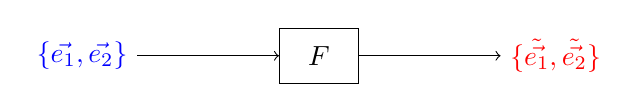
\begin{tikzpicture}[node distance=18mm]
    \node (in) {$\color{blue}\{\vec{e_1}, \vec{e_2}\}$};
    \node[draw, rectangle, minimum width=10mm, minimum height=7mm, right=of in] (F) {$F$};
    \node (out) [right=of F] {$\color{red}\{\tilde{\vec{e_1}}, \tilde{\vec{e_2}}\}$};

    \draw[->] (in) -- (F);
    \draw[->] (F) -- (out);
\end{tikzpicture}

\end{center}

\begin{center}
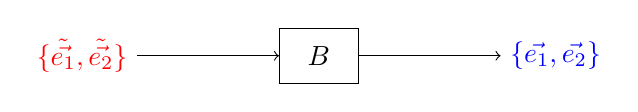
\begin{tikzpicture}[node distance=18mm]
    \node (in) {$\color{red}\{\tilde{\vec{e_1}}, \tilde{\vec{e_2}}\}$};
    \node[draw, rectangle, minimum width=10mm, minimum height=7mm, right=of in] (B) {$B$};
    \node (out) [right=of B] {$\color{blue}\{\vec{e_1}, \vec{e_2}\}$};

    \draw[->] (in) -- (B);
    \draw[->] (B) -- (out);
\end{tikzpicture}

\end{center}

So let's try and check if following the same logic for the vector components, we can move from one coordinate systems to the other, applying the forward matrix, so:\\

\begin{align*}
    F \begingroup\color{blue}\left[ \begin{matrix}
        1 \\
        1.5
    \end{matrix}\right]_{\vec{e_i}}\endgroup =  
    \begin{bmatrix}
    2 & -\frac{1}{2}\\
    1 & \frac{1}{4}
    \end{bmatrix} \begingroup\color{blue}\left[ \begin{matrix}
        1 \\
        1.5
    \end{matrix}\right]_{\vec{e_i}}\endgroup =
    \begin{bmatrix}
    1.25\\
    1.375
    \end{bmatrix}
\end{align*}

This does not seem right, doens't it? Why don't we try to apply the $B$ matrix instead?

\begin{align*}
    B \begingroup\color{blue}\left[ \begin{matrix}
        1 \\
        1.5
    \end{matrix}\right]_{\vec{e_i}}\endgroup =  
    \begin{bmatrix}
    \frac{1}{4} & \frac{1}{2}\\
    -1 & 2
    \end{bmatrix} \begingroup\color{blue}\left[ \begin{matrix}
        1 \\
        1.5
    \end{matrix}\right]_{\vec{e_i}}\endgroup =
    \begin{bmatrix}
    1\\
    2
    \end{bmatrix}
\end{align*}

\textbf{So this tells us that, for basis vectors, forward matrix brings us from old to new, and backward from new to old, but for vector components, it's the opposite, backward matrix brings us from old to new, and forward from new to old}.
This might seem weird at a first look, but it actually makes sense. Let me give you a couple of examples. Let's start with a simple $\color{green}\vec{v}$ in the basis $\color{blue}\vec{e_i}$ and imagine that you want to describe the same vector (invariant) in a different basis $\color{red}\tilde{\vec{e_i}}$, which is only up-scaled by a factor of 2 wrt to the old basis:

\begin{center}
\begin{minipage}[t]{0.48\linewidth}
\centering
\input{figures/03-vector-scaling-old-basis}
\end{minipage}
\hfill
\begin{minipage}[t]{0.48\linewidth}
\centering
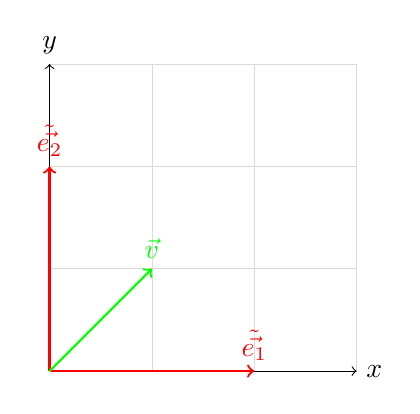
\begin{tikzpicture}[scale=1.3]
  \draw[step=1cm,gray!30,very thin] (0,0) grid (3,3);
  \draw[->] (0,0) -- (3,0) node[right] {$x$};
  \draw[->] (0,0) -- (0,3) node[above] {$y$};
  \draw[->,thick,red] (0,0) -- (2,0) node[above] {$\tilde{\vec{e_1}}$};
  \draw[->,thick,red] (0,0) -- (0,2) node[above] {$\tilde{\vec{e_2}}$};
  \draw[->,thick,green] (0,0) -- (1,1) node[above] {$\vec{v}$};
\end{tikzpicture}

\end{minipage}
\end{center}

If you think about this, as basis vectors scaled up, the vector components have to scale down by the same amount, for the vector itself to be invariant wrt to change of coordinate system. $\color{green}\vec{v}$ "looks" smaller as seen by the new "bigger" coordinate system basis vectors.
Indeed:

\begin{align*}
    \begingroup\color{blue}\left[ \begin{matrix}
        1 \\
        1
    \end{matrix}\right]_{\vec{e_i}}\endgroup & 
    \begingroup\color{red}\left[ \begin{matrix}
        1/2 \\
        1/2
    \end{matrix}\right]_{\tilde{\vec{e_i}}}\endgroup
\end{align*}

The same happens for a simple basis vector rotation:

\begin{center}
\begin{minipage}[t]{0.48\linewidth}
\centering
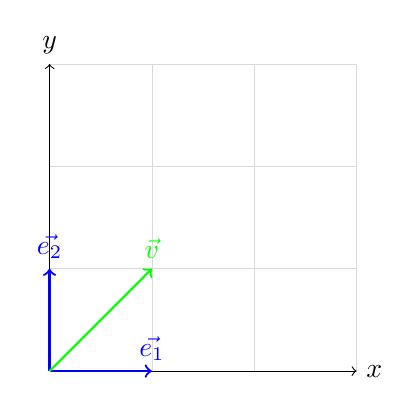
\begin{tikzpicture}[scale=1.3]
  \draw[step=1cm,gray!30,very thin] (0,0) grid (3,3);
  \draw[->] (0,0) -- (3,0) node[right] {$x$};
  \draw[->] (0,0) -- (0,3) node[above] {$y$};
  \draw[->,thick,blue] (0,0) -- (1,0) node[above] {$\vec{e_1}$};
  \draw[->,thick,blue] (0,0) -- (0,1) node[above] {$\vec{e_2}$};
  \draw[->,thick,green] (0,0) -- (1,1) node[above] {$\vec{v}$};
\end{tikzpicture}

\end{minipage}
\hfill
\begin{minipage}[t]{0.48\linewidth}
\centering
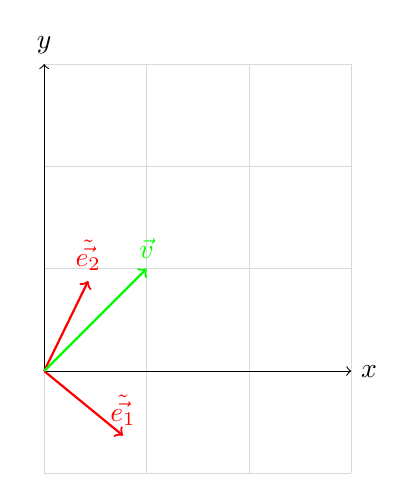
\begin{tikzpicture}[scale=1.3]
  \draw[step=1cm,gray!30,very thin] (0,-1) grid (3,3);
  \draw[->] (0,0) -- (3,0) node[right] {$x$};
  \draw[->] (0,0) -- (0,3) node[above] {$y$};
  \draw[->,thick,red] (0,0) -- (0.77,-0.63) node[above] {$\tilde{\vec{e_1}}$};
  \draw[->,thick,red] (0,0) -- (0.43,0.88) node[above] {$\tilde{\vec{e_2}}$};
  \draw[->,thick,green] (0,0) -- (1,1) node[above] {$\vec{v}$};
\end{tikzpicture}

\end{minipage}
\end{center}

In this case, intuitively and from the picture, it's clearly visible that a clockwise rotation of the basis vectors corresponds to a counter-clockwise rotation of the vector components. \\

Next step would be proving this in more dimentions. We can write the vector as a linear combination of its vector components in two different coordinate systems / basis vectors:

\begin{align*}
    \begingroup\color{green}\vec{v}\endgroup &= \begingroup\color{cyan}v_1\endgroup\begingroup\color{blue}\vec{e_1}\endgroup + \begingroup\color{cyan}v_2\endgroup\begingroup\color{blue}\vec{e_2}\endgroup + \cdots + \begingroup\color{cyan}v_n\endgroup\begingroup\color{blue}\vec{e_n}\endgroup = \sum_{j=1}^{n} \begingroup\color{cyan}v_j\endgroup \begingroup\color{blue}\vec{e_j}\endgroup \\
    \begingroup\color{green}\vec{v}\endgroup &= \begingroup\color{magenta}\tilde{v_1}\endgroup\begingroup\color{red}\tilde{\vec{e_1}}\endgroup + \begingroup\color{magenta}\tilde{v_2}\endgroup\begingroup\color{red}\tilde{\vec{e_2}}\endgroup + \cdots + \begingroup\color{magenta}\tilde{v_n}\endgroup\begingroup\color{red}\tilde{\vec{e_n}}\endgroup = \sum_{j=1}^{n} \begingroup\color{magenta}\tilde{v_j}\endgroup \begingroup\color{red}\tilde{\vec{e_j}}\endgroup
\end{align*}

Bringing back our basis vector forward and backward transformations:

\begin{subequations}
\begin{empheq}[box=\widefbox]{align}
    \begingroup\color{red}\tilde{\vec{e_i}}\endgroup = \sum_{j=1}^{n} F_{ji} \begingroup\color{blue}\vec{e_j}\endgroup \\
    \begingroup\color{blue}\vec{e_i}\endgroup = \sum_{j=1}^{n} B_{ji} \begingroup\color{red}\tilde{\vec{e_j}}\endgroup
\end{empheq}
\end{subequations}

We can write:

\begin{align*}
    \begingroup\color{green}\vec{v}\endgroup &= \sum_{j=1}^{n} \begingroup\color{cyan}v_j\endgroup \begingroup\color{blue}\vec{e_j}\endgroup = \sum_{j=1}^{n} \begingroup\color{cyan}v_j\endgroup \left(\sum_{i=1}^{n} B_{ij} \begingroup\color{red}\tilde{\vec{e_i}}\endgroup\right) = \sum_{i=1}^{n}\left(\sum_{j=1}^{n}B_{ij}\begingroup\color{cyan}v_j\endgroup\right)\begingroup\color{red}\tilde{\vec{e_i}}\endgroup
\end{align*}

As you can see, \textbf{this actually proves that, to move from the old components to the new components, we use the backward transformation matrix}, and \textbf{to move from the new components to the old components, we use the forward transformation matrix}:

\begin{subequations}
\begin{empheq}[box=\widefbox]{align}
    \begingroup\color{magenta}\tilde{v_i}\endgroup = \sum_{j=1}^{n} B_{ij} \begingroup\color{cyan}v_j\endgroup \\
    \begingroup\color{cyan}v_i\endgroup = \sum_{j=1}^{n} F_{ij} \begingroup\color{magenta}\tilde{v_j}\endgroup
\end{empheq}
\end{subequations}

So, summarizing what we've learned so far, we know the transformation rules that basis vectors and vector components obey:

\begin{center}
\begin{minipage}[t]{0.48\linewidth}
\centering
\begin{subequations}
\begin{empheq}[box=\widefbox]{align}
    \begingroup\color{red}\tilde{\vec{e_i}}\endgroup = \sum_{j=1}^{n} F_{ji} \begingroup\color{blue}\vec{e_j}\endgroup \\
    \begingroup\color{blue}\vec{e_i}\endgroup = \sum_{j=1}^{n} B_{ji} \begingroup\color{red}\tilde{\vec{e_j}}\endgroup
\end{empheq}
\end{subequations}
\end{minipage}
\hfill
\begin{minipage}[t]{0.48\linewidth}
\centering
\begin{subequations}
\begin{empheq}[box=\widefbox]{align}
    \begingroup\color{magenta}\tilde{v_i}\endgroup = \sum_{j=1}^{n} B_{ij} \begingroup\color{cyan}v_j\endgroup \\
    \begingroup\color{cyan}v_i\endgroup = \sum_{j=1}^{n} F_{ij} \begingroup\color{magenta}\tilde{v_j}\endgroup
\end{empheq}
\end{subequations}
\end{minipage}
\end{center}

Since the vector components behave contrary to the basis vectors, we say that they are contra-variant. \\
We'll see later indeed, that vectors are contra-variant tensors and from now on, we're going to make a small change in the way we write vector components due to this behavior, and we're writing them with the index on top and not on the bottom:

\begin{align*}
    \begingroup\color{green}\vec{v}\endgroup = \sum_{i=1}^{n} \begingroup\color{cyan}v^i\endgroup \begingroup\color{blue}\vec{e_i}\endgroup = \sum_{i=1}^{n} \begingroup\color{magenta}\tilde{v^i}\endgroup \begingroup\color{red}\tilde{\vec{e_i}}\endgroup
\end{align*}

\section{Covectors and covector components}

You may find in some places, that covectors are defined to be "basically" row vectors, so you may think that's just it, if you have a vector written in column, you flip it and you have a covector, but that's not quite right and simple.

Column-vectors and row-vectors are fundamentally different types of objects.
The reason you may think are basically the same but flipped, is that we normally deal with \emph{orthonormal basis}, which is a basis where all vectors are one unit long and perpendicular to each other. But generally, this is not true in any coordinate system. 

To realize this, we need to think at row vectors as functions acting on column vectors, so let's think about a general covector $\alpha$ acting on a general vector $\vec{v}$:

\begin{equation}
    \alpha(\vec{v}) = \alpha_1 v^1 + \alpha_2 v^2 + \cdots + \alpha_n v^b = \sum_{i=1}^{n}\alpha_i v^i
\end{equation}

Ultimately, a covector is a function that takes an input from a vector space and returns a scalar as output:

\begin{equation}
    \alpha: \textit{V} \to \mathbb{R}
\end{equation}

They obey the linearity rule:
\begin{equation}
    \alpha(n\vec{v} + m\vec{w}) = n\alpha(\vec{v}) + m\alpha(\vec{w})
\end{equation}

How can we visualized these covectors though? There's a nice way of doing it and we can start by thinking about a generic 2D covector as a function on two variables $x$ and $y$:

\begin{align*}
    \begin{bmatrix}
    2 & 1
    \end{bmatrix} \left(
        \begin{bmatrix}
        x \\
        y
    \end{bmatrix}
    \right) = 2x + 1y
\end{align*}

So how do we visualize a function of two variables that produces one output?
This is very similar to what tophographers do to visualize on a piece of 2D paper a topographic map of some mountains and valley.
This is done by drawing curves of constant elevation value. And by looking at a mpa like this, we know that when we see these lines very close together they represent a place where the elevation changes very steeply, whereas where they are less dense, the elevation does not change so steeply.\\

Continuing with out example, we can start asking, where is this function equal to zero? $2x + 1y = 0$ ? This is the line $y = -2x$, same we can do for 1, 2, 3 and for negative as well.

\begin{center}
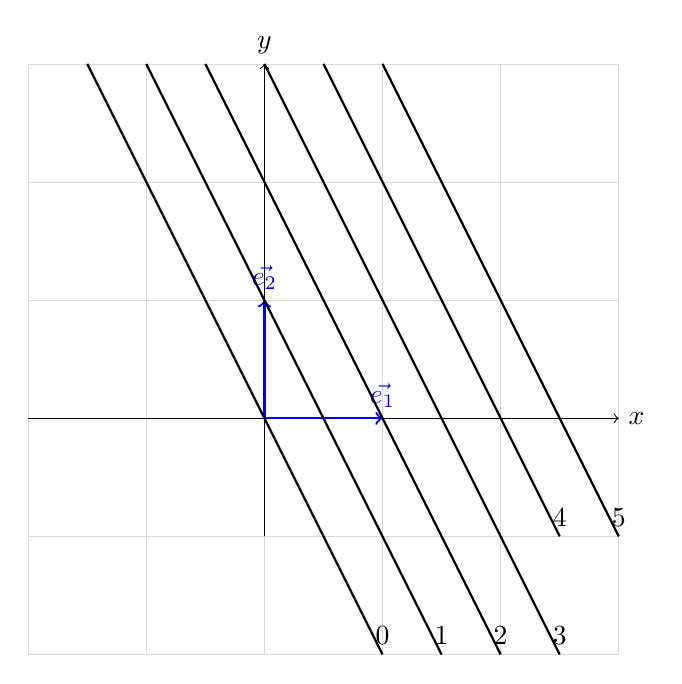
\begin{tikzpicture}[scale=1.5]
  \draw[step=1cm,gray!30,very thin] (-2,-2) grid (3,3);
  \draw[->] (-2,0) -- (3,0) node[right] {$x$};
  \draw[->] (0,-1) -- (0,3) node[above] {$y$};
  \draw[->,thick,blue] (0,0) -- (1,0) node[above] {$\vec{e_1}$};
  \draw[->,thick,blue] (0,0) -- (0,1) node[above] {$\vec{e_2}$};
  \draw[black,thick,domain=-1.5:1] plot (\x,{-2*\x}) node[above] {0};
  \draw[black,thick,domain=-1:1.5] plot (\x,{-2*\x+1}) node[above] {1};
  \draw[black,thick,domain=-0.5:2] plot (\x,{-2*\x+2}) node[above] {2};
  \draw[black,thick,domain=0:2.5] plot (\x,{-2*\x+3}) node[above] {3};
  \draw[black,thick,domain=0.5:2.5] plot (\x,{-2*\x+4}) node[above] {4};
  \draw[black,thick,domain=1:3] plot (\x,{-2*\x+5}) node[above] {5};
\end{tikzpicture}

\end{center}

The stack is increasing towards the upper right so it has a direction towards north-east in our case.

You can actually think about a covector $\alpha$ acting on a vector $\vec{v}$ as giving a scalar output, equals to the number of times the vector pierces one of the covector's lines.

Now what happens if we scale up the covector, let's say by a factor of 2?
We basically make is much denser, hence the vector will pierce the lines double the time it did before.
And the result would be the same if we choose instead, of scaling up the vector by 2, as the vector will then pierce a double number of lines, being its magnitude longer.

Let's continue on how we can visualize two covector addition.

\begin{align*}
    \beta(\begingroup\color{orange}\vec{v}\endgroup) = 3\\
    \gamma(\begingroup\color{orange}\vec{v}\endgroup) = 2
\end{align*}

\begin{center}
\begin{minipage}[t]{0.32\linewidth}
\centering
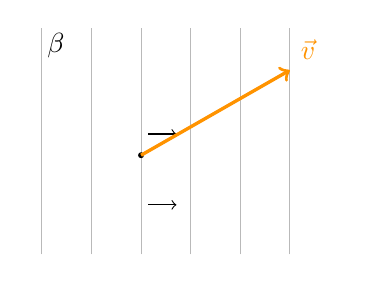
\begin{tikzpicture}[scale=0.9]
  % beta: vertical family of lines
  \clip (-2.2,-1.6) rectangle (2.2,1.6);
  \foreach \x in {-2,-1.3,...,2} {
    \draw[gray!55, line width=0.35pt] (\x,-1.6) -- (\x,1.6);
  }
  % direction markers
  \draw[->, black, line width=0.4pt] (-0.5,-0.9) -- (-0.1,-0.9);
  \draw[->, black, line width=0.4pt] (-0.5,0.1) -- (-0.1,0.1);

  % vector v
  \fill[black] (-0.6,-0.2) circle (1.2pt);
  \draw[->, very thick, orange!85!yellow] (-0.6,-0.2) -- (1.5,1.0) node[above right] {$\vec{v}$};

  \node at (-1.8,1.35) {$\beta$};
\end{tikzpicture}

\end{minipage}
\hfill
\begin{minipage}[t]{0.32\linewidth}
\centering
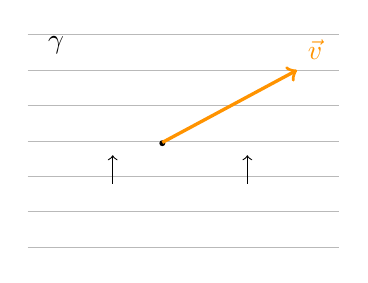
\begin{tikzpicture}[scale=0.9]
  % gamma: horizontal family of lines
  \clip (-2.2,-1.6) rectangle (2.2,1.6);
  \foreach \y in {-1.5,-1.0,...,1.5} {
    \draw[gray!55, line width=0.35pt] (-2.2,\y) -- (2.2,\y);
  }
  % direction markers
  \draw[->, black, line width=0.4pt] (-1.0,-0.6) -- (-1.0,-0.2);
  \draw[->, black, line width=0.4pt] (0.9,-0.6) -- (0.9,-0.2);

  % vector v
  \fill[black] (-0.3,-0.03) circle (1.2pt);
  \draw[->, very thick, orange!85!yellow] (-0.3,-0.02) -- (1.6,1.0) node[above right] {$\vec{v}$};

  \node at (-1.8,1.35) {$\gamma$};
\end{tikzpicture}

\end{minipage}
\hfill
\begin{minipage}[t]{0.32\linewidth}
\centering
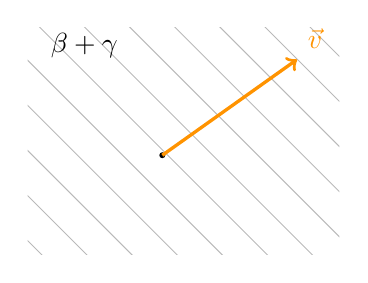
\begin{tikzpicture}[scale=0.9]
  % beta + gamma: diagonal family of lines
  \clip (-2.2,-1.6) rectangle (2.2,1.6);
  \begin{scope}[rotate=45]
    \foreach \x in {-3,-2.55,...,3} {
      \draw[gray!55, line width=0.35pt] (\x,-3) -- (\x,3);
    }
  \end{scope}

  % vector v
  \fill[black] (-0.3,-0.2) circle (1.2pt);
  \draw[->, very thick, orange!85!yellow] (-0.3,-0.2) -- (1.6,1.15) node[above right] {$\vec{v}$};

  \node at (-1.4,1.35) {$\beta + \gamma$};
\end{tikzpicture}

\end{minipage}
\end{center}

The diagrams are not perfect, but a sum of covectors $\beta$ and $\gamma$ would show as a stack with the same density as $\beta$ in the beta-direction, and same density as $\gamma$ in the gamma-direction, which in this case would visualize as a NE-pointing stack, and since $\beta$ has an horizontal density of 3 and $\gamma$ a vertical density of 2, the sum will simply be the vector piercing the lines 5 times.

\begin{align*}
    \left(\beta + \gamma\right)(\begingroup\color{orange}\vec{v}\endgroup) = 5\\
    \left(\beta + \gamma\right)(\begingroup\color{orange}\vec{v}\endgroup) = \beta(\begingroup\color{orange}\vec{v}\endgroup) + \gamma(\begingroup\color{orange}\vec{v}\endgroup)
\end{align*}

Summing up, we've seen that for covectors, we also are able to scale them, and perform addition, and that gives us a hint about the fact that covectors are actually part of a Vector space.\\
We have that the set of covectors that act on vectors in $V$ form a new vector space called the \emph{dual space} $V^*$, with its own set of addition and scalar operations:

\begin{align*}
    \left(V, S, +, \cdot \right) \\
    \left(V^*, S, \begingroup\color{red}+, \cdot\endgroup \right)
\end{align*}

The elements of $V^*$ are covectors, which are functions that go from $\textit{V}$ to the real numbers $\mathbb{R}$, with their own addition and scaling rules:

\begin{align*}
    \left(n\begingroup\color{red}\cdot\endgroup \alpha\right)\left(\begingroup\color{orange}\vec{v}\endgroup\right) = n\alpha\left(\begingroup\color{orange}\vec{v}\endgroup\right) \\
    \left(\beta \begingroup\color{red}+\endgroup \gamma\right)(\begingroup\color{orange}\vec{v}\endgroup) = \beta(\begingroup\color{orange}\vec{v}\endgroup) + \gamma(\begingroup\color{orange}\vec{v}\endgroup)
\end{align*}

As per vectors, covectors are also invariant, they're purely geometric object, independend of the reference frame/coordinate system used to describe them.
Their components though, exactly like vector components, are not invariant.

When we write a column vector, for example, as follows, we represent it by how much of each basis vector I need to make this vector, so as a linear combination of the "scaled" basis vectors (scaled by the vector components values):

\begin{equation}
    \left[ \begin{matrix}
        2 \\
        1
    \end{matrix}\right]_{\color{blue}\vec{e_i}} \text{ we mean } 2\begingroup\color{blue}\vec{e_1}\endgroup + 1\begingroup\color{blue}\vec{e_2}\endgroup
\end{equation}

But what does it mean to do this for covectors? Which are functions? Like if I write down 

\begin{equation}
    \left[ \begin{matrix}
        2 & 1
    \end{matrix}\right]
\end{equation}

This is not as intuitive because remember that covectors do not live in the same vector space, they live in the dual vector space, and they are functions from vectors to real numbers, so we can't use basis vectors in $V$ to represent covectors of $V^*$.\\

What we can do is intruduce two special covectors, such that, considering the basis $\color{blue} \{\vec{e_1}, \vec{e_2}\}$ for $V$:

\begin{align*}
    \begingroup\color{violet}\epsilon^1\endgroup\left(\begingroup\color{blue}\vec{e_1}\endgroup\right) &= 1 & \begingroup\color{violet}\epsilon^1\endgroup\left(\begingroup\color{blue}\vec{e_2}\endgroup\right) &= 0 \\
    \begingroup\color{violet}\epsilon^2\endgroup\left(\begingroup\color{blue}\vec{e_1}\endgroup\right) &= 0 & \begingroup\color{violet}\epsilon^2\endgroup\left(\begingroup\color{blue}\vec{e_2}\endgroup\right) &= 1
\end{align*}

so basically:

\begin{equation}
    \begingroup\color{violet}\epsilon^i\endgroup\left(\begingroup\color{blue}\vec{e_j}\endgroup\right) = \delta^i{}_j = \begin{cases}
            1, &         \text{if } i=j,\\
            0, &         \text{if } i\neq j.
    \end{cases}
\end{equation}

What happens when we apply such covectors to a generic vector?

\begin{align*}
    \begingroup\color{violet}\epsilon^1\endgroup\left(\begingroup\color{orange}\vec{v}\endgroup\right) = \begingroup\color{violet}\epsilon^1\endgroup\left(v^1 \begingroup\color{blue}\vec{e_1}\endgroup + v^2 \begingroup\color{blue}\vec{e_2}\endgroup\right) = v^1 \\
    \begingroup\color{violet}\epsilon^2\endgroup\left(\begingroup\color{orange}\vec{v}\endgroup\right) = \begingroup\color{violet}\epsilon^2\endgroup\left(v^1 \begingroup\color{blue}\vec{e_1}\endgroup + v^2 \begingroup\color{blue}\vec{e_2}\endgroup\right) = v^2 \\
    \begingroup\color{violet}\epsilon^i\endgroup\left(\begingroup\color{orange}\vec{v}\endgroup\right) = v^i
\end{align*}

So what these covectors are doing, is projecting out vector components.

\begin{center}
\begin{minipage}[t]{0.48\linewidth}
\centering
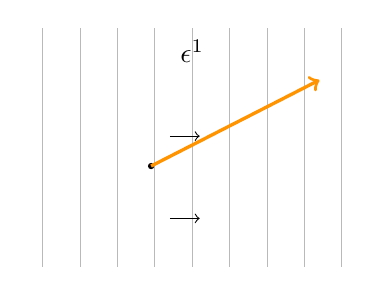
\begin{tikzpicture}[scale=0.95]
  \clip (-2.2,-1.6) rectangle (2.2,1.6);

  % epsilon^1: vertical family of lines
  \foreach \x in {-2,-1.5,...,2} {
    \draw[gray!55, line width=0.35pt] (\x,-1.6) -- (\x,1.6);
  }

  % direction markers
  \draw[->, black, line width=0.4pt] (-0.3,-0.95) -- (0.1,-0.95);
  \draw[->, black, line width=0.4pt] (-0.3,0.15) -- (0.1,0.15);

  % vector v
  \fill[black] (-0.55,-0.25) circle (1.2pt);
  \draw[->, very thick, orange!85!yellow] (-0.55,-0.25) -- (1.7,0.9);

  \node[anchor=south] at (0,1.0) {$\epsilon^1$};
\end{tikzpicture}

\end{minipage}
\hfill
\begin{minipage}[t]{0.48\linewidth}
\centering
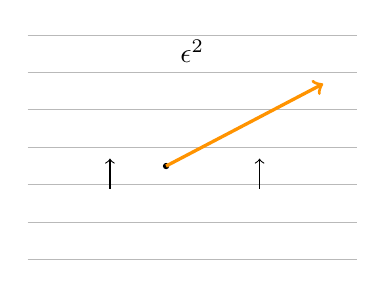
\begin{tikzpicture}[scale=0.95]
  \clip (-2.2,-1.6) rectangle (2.2,1.6);

  % epsilon^2: horizontal family of lines
  \foreach \y in {-1.5,-1.0,...,1.5} {
    \draw[gray!55, line width=0.35pt] (-2.2,\y) -- (2.2,\y);
  }

  % direction markers
  \draw[->, black, line width=0.4pt] (-1.1,-0.55) -- (-1.1,-0.15);
  \draw[->, black, line width=0.4pt] (0.9,-0.55) -- (0.9,-0.15);

  % vector v
  \fill[black] (-0.35,-0.25) circle (1.2pt);
  \draw[->, very thick, orange!85!yellow] (-0.35,-0.25) -- (1.75,0.85);

  \node[anchor=south] at (0,1.0) {$\epsilon^2$};
\end{tikzpicture}

\end{minipage}
\end{center}

Let's now generalize and apply a general covector $\alpha$ to a vector $\color{orange}\vec{v}$:

\begin{align*}
    \alpha\left(\begingroup\color{orange}\vec{v}\endgroup\right) = \alpha\left(v^1 \begingroup\color{blue}\vec{e_1}\endgroup + v^2 \begingroup\color{blue}\vec{e_2}\endgroup\right) = v^1\alpha\left(\begingroup\color{blue}\vec{e_1}\endgroup\right) + v^2 \left(\begingroup\color{blue}\vec{e_2}\endgroup\right)
\end{align*}

We can write the components $v_i = \begingroup\color{violet}\epsilon^i\endgroup\left(\begingroup\color{orange}\vec{v}\endgroup\right)$ so that:

\begin{align*}
    \alpha\left(\begingroup\color{orange}\vec{v}\endgroup\right) = \begingroup\color{violet}\epsilon^1\endgroup\left(\begingroup\color{orange}\vec{v}\endgroup\right)\alpha\left(\begingroup\color{blue}\vec{e_1}\endgroup\right) + \begingroup\color{violet}\epsilon^2\endgroup\left(\begingroup\color{orange}\vec{v}\endgroup\right) \alpha\left(\begingroup\color{blue}\vec{e_2}\endgroup\right)
\end{align*}

We define $\alpha\left(\begingroup\color{blue}\vec{e_1}\endgroup\right) = \alpha_1$ and $\alpha\left(\begingroup\color{blue}\vec{e_2}\endgroup\right) = \alpha_2$ so that:

\begin{align*}
    \alpha\left(\begingroup\color{orange}\vec{v}\endgroup\right) &= \alpha_1\begingroup\color{violet}\epsilon^1\endgroup\left(\begingroup\color{orange}\vec{v}\endgroup\right) + \alpha_2\begingroup\color{violet}\epsilon^2\endgroup\left(\begingroup\color{orange}\vec{v}\endgroup\right) \\
    \alpha\left(\begingroup\color{orange}\vec{v}\endgroup\right) &= \left(\alpha_1\begingroup\color{violet}\epsilon^1\endgroup + \alpha_2\begingroup\color{violet}\epsilon^2\endgroup\right)\left(\begingroup\color{orange}\vec{v}\endgroup\right) \\
    \alpha &= \alpha_1\begingroup\color{violet}\epsilon^1\endgroup + \alpha_2\begingroup\color{violet}\epsilon^2\endgroup
\end{align*}

We've now written a covector $\alpha$ as linear combination of our epsilon covectors defined above. \textbf{What this means is that the $\epsilon$ covectors form a basis for the dual vector space $V^*$} and we call this $\epsilon$ the dual basis because they're a basis for the dual vector space $V^*$.\\

We may try to understand this visually and geometrically, since so far we derived this algebraically.

\begin{center}
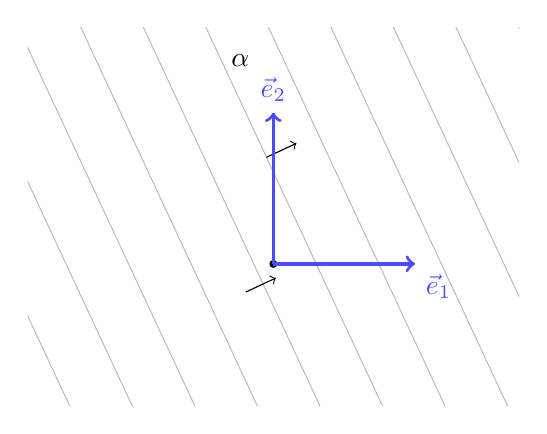
\begin{tikzpicture}[scale=1.2]
  \clip (-2.6,-2.0) rectangle (2.6,2.0);

  % Diagonal level sets for a generic covector alpha
  \begin{scope}[rotate=25]
    \foreach \x in {-4,-3.4,...,4} {
      \draw[gray!55, line width=0.35pt] (\x,-4) -- (\x,4);
    }
    % small direction markers (indicating increasing values)
    \draw[->, black, line width=0.4pt] (-0.6,-0.6) -- (-0.25,-0.6);
    \draw[->, black, line width=0.4pt] (0.2,0.6) -- (0.55,0.6);
  \end{scope}

  % Basis vectors e1, e2
  \fill[black] (0,-0.5) circle (1.2pt);
  \draw[->, very thick, blue!70] (0,-0.5) -- (1.5,-0.5) node[below right] {$\vec{e}_1$};
  \draw[->, very thick, blue!70] (0,-0.5) -- (0,1.1) node[above] {$\vec{e}_2$};

  % labels
  \node at (-0.35,1.65) {$\alpha$};
\end{tikzpicture}

\end{center}

We can get the components of $\alpha$ by applying the covector to the basis vectors: $\alpha\left(\begingroup\color{blue}\vec{e_1}\endgroup\right) = \alpha_1$ and $\alpha\left(\begingroup\color{blue}\vec{e_2}\endgroup\right) = \alpha_2$.
In terms of the dual basis $\{\epsilon^1,\epsilon^2\}$ we can visualize the decomposition
\[
  \alpha = \alpha_1\,\epsilon^1 + \alpha_2\,\epsilon^2.
\]

\begin{center}
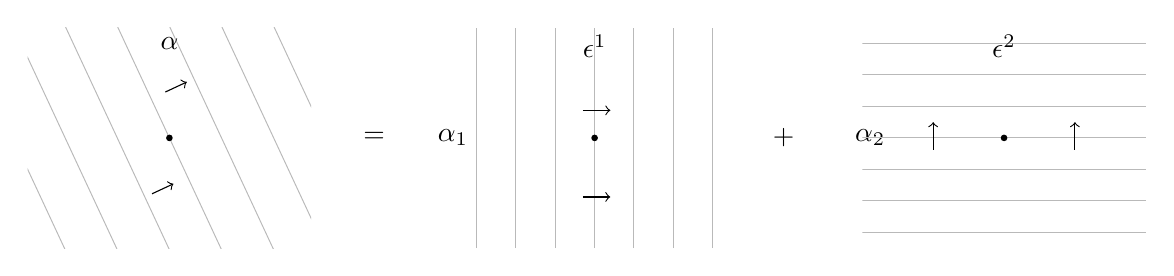
\begin{tikzpicture}[scale=1.0]
  % Layout anchors
  \node (A) at (0,0) {};

  % -------- left: alpha --------
  \begin{scope}[shift={(-5.2,0)}]
    \clip (-1.8,-1.4) rectangle (1.8,1.4);
    \begin{scope}[rotate=25]
      \foreach \x in {-3,-2.4,...,3} {
        \draw[gray!55, line width=0.35pt] (\x,-3) -- (\x,3);
      }
      \draw[->, black, line width=0.4pt] (-0.5,-0.55) -- (-0.2,-0.55);
      \draw[->, black, line width=0.4pt] (0.2,0.55) -- (0.5,0.55);
    \end{scope}
    \fill[black] (0,0) circle (1.2pt);
    \node[anchor=south] at (0,1.0) {$\alpha$};
  \end{scope}

  % -------- equals sign --------
  \node at (-2.6,0) {$=$};

  % -------- middle: alpha1 * epsilon1 --------
  \node at (-1.6,0) {$\alpha_1$};
  \begin{scope}[shift={(0.2,0)}]
    \clip (-1.8,-1.4) rectangle (1.8,1.4);
    \foreach \x in {-2,-1.5,...,2} {
      \draw[gray!55, line width=0.35pt] (\x,-1.4) -- (\x,1.4);
    }
    \draw[->, black, line width=0.4pt] (-0.15,-0.75) -- (0.2,-0.75);
    \draw[->, black, line width=0.4pt] (-0.15,0.35) -- (0.2,0.35);
    \fill[black] (0,0) circle (1.2pt);
    \node[anchor=south] at (0,0.9) {$\epsilon^1$};
  \end{scope}

  % -------- plus sign --------
  \node at (2.6,0) {$+$};

  % -------- right: alpha2 * epsilon2 --------
  \node at (3.7,0) {$\alpha_2$};
  \begin{scope}[shift={(5.4,0)}]
    \clip (-1.8,-1.4) rectangle (1.8,1.4);
    \foreach \y in {-1.2,-0.8,...,1.2} {
      \draw[gray!55, line width=0.35pt] (-1.8,\y) -- (1.8,\y);
    }
    \draw[->, black, line width=0.4pt] (-0.9,-0.15) -- (-0.9,0.2);
    \draw[->, black, line width=0.4pt] (0.9,-0.15) -- (0.9,0.2);
    \fill[black] (0,0) circle (1.2pt);
    \node[anchor=south] at (0,0.9) {$\epsilon^2$};
  \end{scope}
\end{tikzpicture}

\end{center}

The process is, we start with our vector basis $\color{blue}\vec{e_1}, \vec{e_2}$, then using this $\begingroup\color{violet}\epsilon^i\endgroup\left(\begingroup\color{blue}\vec{e_j}\endgroup\right) = \delta^i{}_j$, we get the dual covector basis, and then using those we can express any covector as a combination of the dual basis. \\ 

Remember though, that these $\epsilon$ covector basis is not the only one we can use to express $\alpha$.
We can start with a different vector basis, $\color{red}\tilde{\vec{e_1}}, \tilde{\vec{e_2}}$ and then applying the rule $\begingroup\color{red}\tilde{\epsilon^i}\endgroup\left(\begingroup\color{red}\tilde{\vec{e_j}}\endgroup\right) = \delta^i{}_j$ we get another dual vector basis, that can be used to express the same $\alpha$ in a different covector basis.

Allright, so now, let's say we have a covector $\alpha = 2\begingroup\color{blue}\epsilon^1\endgroup + 1\begingroup\color{blue}\epsilon^2\endgroup$ represented in the old covector basis $\color{blue}\epsilon^i$:

\begin{equation}
    \color{blue}\left[ \begin{matrix}
        2 & 1
    \end{matrix}\right]_{\epsilon^i}
\end{equation}

which means they have components:

\begin{align*}
    \alpha\left(\begingroup\color{blue}\vec{e_1}\endgroup\right) = 2\\
    \alpha\left(\begingroup\color{blue}\vec{e_2}\endgroup\right) = 1
\end{align*}

What would these components look like in the new covector basis $\color{red}\tilde{\epsilon^i}$ ?

For this we need to apply the covector $\alpha$ to the new basis vectors:

\begin{align*}
    \alpha\left(\begingroup\color{red}\tilde{\vec{e_1}}\endgroup\right) = \begingroup\color{magenta}\tilde{\alpha_1}\endgroup\\
    \alpha\left(\begingroup\color{red}\tilde{\vec{e_2}}\endgroup\right) = \begingroup\color{magenta}\tilde{\alpha_2}\endgroup
\end{align*}

And taking this coordinate systems in example:

\begin{center}
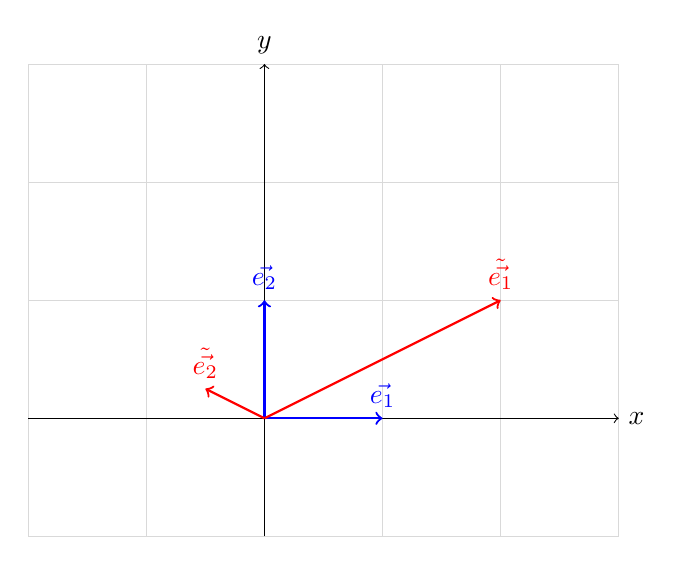
\begin{tikzpicture}[scale=1.5]
  \draw[step=1cm,gray!30,very thin] (-2,-1) grid (3,3);
  \draw[->] (-2,0) -- (3,0) node[right] {$x$};
  \draw[->] (0,-1) -- (0,3) node[above] {$y$};
  \draw[->,thick,blue] (0,0) -- (1,0) node[above] {$\vec{e_1}$};
  \draw[->,thick,blue] (0,0) -- (0,1) node[above] {$\vec{e_2}$};
  \draw[->,thick,red] (0,0) -- (2,1) node[above] {$\tilde{\vec{e_1}}$};
  \draw[->,thick,red] (0,0) -- (-0.5,0.25) node[above] {$\tilde{\vec{e_2}}$};
\end{tikzpicture}

\end{center}

We see that $\begingroup\color{red}\tilde{\vec{e_1}}\endgroup = \left(2\begingroup\color{blue}\vec{e_1}\endgroup + 1\begingroup\color{blue}\vec{e_2}\endgroup\right)$ and $\begingroup\color{red}\tilde{\vec{e_2}}\endgroup = \left(-1/2\begingroup\color{blue}\vec{e_1}\endgroup + 1/4\begingroup\color{blue}\vec{e_2}\endgroup\right)$ so:

\begin{align*}
    \begingroup\color{magenta}\tilde{\alpha_1}\endgroup &= 
    \alpha\left(\begingroup\color{red}\tilde{\vec{e_1}}\endgroup\right) = \alpha\left(2\begingroup\color{blue}\vec{e_1}\endgroup + 1\begingroup\color{blue}\vec{e_2}\endgroup\right) = 5 \\
    \begingroup\color{magenta}\tilde{\alpha_2}\endgroup &= 
    \alpha\left(\begingroup\color{red}\tilde{\vec{e_2}}\endgroup\right) = \alpha\left(-1/2\begingroup\color{blue}\vec{e_1}\endgroup + 1/4\begingroup\color{blue}\vec{e_2}\endgroup\right) = -3/4
\end{align*}

\begin{align*}
    \color{blue}\left[ \begin{matrix}
        2 & 1
    \end{matrix}\right]_{\epsilon^i} && \color{red}\left[ \begin{matrix}
        5 & -3/4
    \end{matrix}\right]_{\tilde{\epsilon^i}}
\end{align*}

Remember what were the $F$ and $B$ matrices? \textbf{If you make your calculation, you will see that for covector components, forward brings from old to new, and backward brings from new to old}:

\begin{align*}
    \begingroup\color{blue}\left[ \begin{matrix}
        2 & 1
    \end{matrix}\right]_{\epsilon^i}\endgroup F &= 
    \begingroup\color{blue}\left[ \begin{matrix}
        2 & 1
    \end{matrix}\right]_{\epsilon^i}\endgroup
    \begin{bmatrix}
    2 & -1/2\\
    1 & 1/4
    \end{bmatrix} = \color{red}\left[ \begin{matrix}
        5 & -3/4
    \end{matrix}\right]_{\tilde{\epsilon^i}} \\
    \begingroup\color{red}\left[ \begin{matrix}
        5 & -3/4
    \end{matrix}\right]_{\tilde{\epsilon^i}}\endgroup B &=
    \begingroup\color{red}\left[ \begin{matrix}
        5 & -3/4
    \end{matrix}\right]_{\tilde{\epsilon^i}}\endgroup
    \begin{bmatrix}
    1/4 & 1/2\\
    -1 & 2
    \end{bmatrix} = \begingroup\color{blue}\left[ \begin{matrix}
        2 & 1
    \end{matrix}\right]_{\epsilon^i}\endgroup
\end{align*}

This is actually the opposite of what we've found for vector components under a change of basis.
\textbf{This is why we can't just flip column vectors to row vectors to get covectors.} 
It works in an orthonormal basis, like the $\color{blue}\vec{e_i}$ and correspondent dual basis defined by $\color{blue}\epsilon^i$.
But it does not work in the new voctor basis $\color{red}\tilde{\vec{e_i}}$ and correspondent covector basis $\color{red}\tilde{\epsilon^i}$.\\

Like we did for vectors bafore, we've gone from old basis vectors to new basis vectors and we found that that requires the forward mateix $F$.

Now we want to do something similar for the covector basis, we want to go from an old covector basis $\color{blue}\epsilon^i$ to a new covector basis $\color{red}\tilde{\epsilon^i}$.

\begin{equation}
    \begingroup\color{red}\tilde{\epsilon^1}\endgroup = Q_{11} \begingroup\color{blue}\epsilon^1\endgroup + Q_{12} \begingroup\color{blue}\epsilon^2\endgroup
\end{equation}
\begin{equation}
    \begingroup\color{red}\tilde{\epsilon^2}\endgroup = Q_{21} \begingroup\color{blue}\epsilon^1\endgroup + Q_{22} \begingroup\color{blue}\epsilon^2\endgroup
\end{equation}

To find the coefficients, we start by applying:

\begin{align*}
    \begingroup\color{red}\tilde{\epsilon^1}\endgroup\left(\begingroup\color{blue}\vec{e_1}\endgroup\right) &= Q_{11} \begingroup\color{blue}\epsilon^1\endgroup\left(\begingroup\color{blue}\vec{e_1}\endgroup\right) + Q_{12} \begingroup\color{blue}\epsilon^2\endgroup\left(\begingroup\color{blue}\vec{e_1}\endgroup\right) = Q_{11} \\
    \begingroup\color{red}\tilde{\epsilon^1}\endgroup\left(\begingroup\color{blue}\vec{e_2}\endgroup\right) &= Q_{11} \begingroup\color{blue}\epsilon^1\endgroup\left(\begingroup\color{blue}\vec{e_2}\endgroup\right) + Q_{12} \begingroup\color{blue}\epsilon^2\endgroup\left(\begingroup\color{blue}\vec{e_2}\endgroup\right) = Q_{12}
\end{align*}

Given this, we can re-write:

\begin{align*}
    \begingroup\color{red}\tilde{\epsilon^1}\endgroup = \begingroup\color{red}\tilde{\epsilon^1}\endgroup\left(\begingroup\color{blue}\vec{e_1}\endgroup\right) \begingroup\color{blue}\epsilon^1\endgroup + \begingroup\color{red}\tilde{\epsilon^1}\endgroup\left(\begingroup\color{blue}\vec{e_2}\endgroup\right) \begingroup\color{blue}\epsilon^2\endgroup
\end{align*}

Now if we bring back our backward transformation, we know that:

\begin{align*}
    \begingroup\color{blue}\vec{e_1}\endgroup &= 1/4 \begingroup\color{red}\tilde{\vec{e_1}}\endgroup -1 \begingroup\color{red}\tilde{\vec{e_2}}\endgroup\\
    \begingroup\color{blue}\vec{e_2}\endgroup &= 1/2 \begingroup\color{red}\tilde{\vec{e_1}}\endgroup + 2 \begingroup\color{red}\tilde{\vec{e_2}}\endgroup
\end{align*}

We can type down:

\begin{align*}
    \begingroup\color{red}\tilde{\epsilon^1}\endgroup &= \begingroup\color{red}\tilde{\epsilon^1}\endgroup\left(1/4 \begingroup\color{red}\tilde{\vec{e_1}}\endgroup -1 \begingroup\color{red}\tilde{\vec{e_2}}\endgroup\right) \begingroup\color{blue}\epsilon^1\endgroup + \begingroup\color{red}\tilde{\epsilon^1}\endgroup\left(1/2 \begingroup\color{red}\tilde{\vec{e_1}}\endgroup + 2 \begingroup\color{red}\tilde{\vec{e_2}}\endgroup\right) \begingroup\color{blue}\epsilon^2\endgroup\\
    \begingroup\color{red}\tilde{\epsilon^1}\endgroup &= \left(1/4 \begingroup\color{red}\tilde{\epsilon^1}\endgroup \left(\begingroup\color{red}\tilde{\vec{e_1}}\endgroup\right) -1 \begingroup\color{red}\tilde{\epsilon^1}\endgroup \left(\begingroup\color{red}\tilde{\vec{e_2}}\endgroup\right)\right)\begingroup\color{blue}\epsilon^1\endgroup + \left(1/2 \begingroup\color{red}\tilde{\epsilon^1}\endgroup \left(\begingroup\color{red}\tilde{\vec{e_1}}\endgroup\right) +2 \begingroup\color{red}\tilde{\epsilon^1}\endgroup \left(\begingroup\color{red}\tilde{\vec{e_2}}\endgroup\right)\right)\begingroup\color{blue}\epsilon^2\endgroup\\
    \begingroup\color{red}\tilde{\epsilon^1}\endgroup &= 1/4\begingroup\color{blue}\epsilon^1\endgroup + 1/2\begingroup\color{blue}\epsilon^2\endgroup \\\\
    \begingroup\color{red}\tilde{\epsilon^2}\endgroup &= \begingroup\color{red}\tilde{\epsilon^2}\endgroup\left(1/4 \begingroup\color{red}\tilde{\vec{e_1}}\endgroup -1 \begingroup\color{red}\tilde{\vec{e_2}}\endgroup\right) \begingroup\color{blue}\epsilon^1\endgroup + \begingroup\color{red}\tilde{\epsilon^2}\endgroup\left(1/2 \begingroup\color{red}\tilde{\vec{e_1}}\endgroup + 2 \begingroup\color{red}\tilde{\vec{e_2}}\endgroup\right) \begingroup\color{blue}\epsilon^2\endgroup\\
    \begingroup\color{red}\tilde{\epsilon^2}\endgroup &= \left(1/4 \begingroup\color{red}\tilde{\epsilon^2}\endgroup \left(\begingroup\color{red}\tilde{\vec{e_1}}\endgroup\right) -1 \begingroup\color{red}\tilde{\epsilon^2}\endgroup \left(\begingroup\color{red}\tilde{\vec{e_2}}\endgroup\right)\right)\begingroup\color{blue}\epsilon^1\endgroup + \left(1/2 \begingroup\color{red}\tilde{\epsilon^2}\endgroup \left(\begingroup\color{red}\tilde{\vec{e_1}}\endgroup\right) +2 \begingroup\color{red}\tilde{\epsilon^2}\endgroup \left(\begingroup\color{red}\tilde{\vec{e_2}}\endgroup\right)\right)\begingroup\color{blue}\epsilon^2\endgroup\\
    \begingroup\color{red}\tilde{\epsilon^2}\endgroup &= -1\begingroup\color{blue}\epsilon^1\endgroup + 2\begingroup\color{blue}\epsilon^2\endgroup
\end{align*}

If you notice, this is quite familiar to the backward transformation, that means that to go from the old dual basis to the new dual basis, we use the $B$ matrix.
This is also valid for every dimension, we'll leave this proof out, but this is the result, showing both the already seen vector basis transformation, and this new dual covector basis one:

\begin{center}
\begin{minipage}[t]{0.48\linewidth}
\centering
\begin{subequations}
\begin{empheq}[box=\widefbox]{align}
    \begingroup\color{red}\tilde{\vec{e_j}}\endgroup = \sum_{j=1}^{n} F_{ij} \begingroup\color{blue}\vec{e_i}\endgroup \\
    \begingroup\color{blue}\vec{e_j}\endgroup = \sum_{j=1}^{n} B_{ij} \begingroup\color{red}\tilde{\vec{e_i}}\endgroup
\end{empheq}
\end{subequations}
\end{minipage}
\hfill
\begin{minipage}[t]{0.48\linewidth}
\centering
\begin{subequations}
\begin{empheq}[box=\widefbox]{align}
    \begingroup\color{red}\tilde{\epsilon^i}\endgroup = \sum_{j=1}^{n} B_{ij} \begingroup\color{blue}\epsilon^j\endgroup \\
    \begingroup\color{blue}\epsilon^i\endgroup = \sum_{j=1}^{n} F_{ij} \begingroup\color{red}\tilde{\epsilon^j}\endgroup
\end{empheq}
\end{subequations}
\end{minipage}
\end{center}

That's why we write covector indeces on top, because the transorm like vector components, opposite to the basis vectors (i.e. contra-variantly)\\

With this now, we can also show how covector components transform:

\begin{subequations}
\begin{empheq}[box=\widefbox]{align}
    \begingroup\color{magenta}\tilde{\alpha_j}\endgroup = \sum_{i=1}^{n} F_{ij} \begingroup\color{cyan}\alpha_i\endgroup \\
    \begingroup\color{cyan}\alpha_j\endgroup = \sum_{i=1}^{n} B_{ij} \begingroup\color{magenta}\tilde{\alpha_j}\endgroup
\end{empheq}
\end{subequations}

Covector components transform in the same way vector basis do.

To summarize all the transformation rules so far:

\[
\begin{array}{cc}
\fbox{
\begin{aligned}
\begingroup\color{red}\tilde{\vec e}_j\endgroup &= \sum_{i=1}^n F_{ij}\,\begingroup\color{blue}\vec e_i\endgroup \\
\begingroup\color{blue}\vec e_j\endgroup &= \sum_{i=1}^n B_{ij}\,\begingroup\color{red}\tilde{\vec e}_i\endgroup
\end{aligned}
}
&
\fbox{
\begin{aligned}
\begingroup\color{red}\tilde{\epsilon}^{\,i}\endgroup &= \sum_{j=1}^n B_{ij}\,\begingroup\color{blue}\epsilon^{j}\endgroup \\
\begingroup\color{blue}\epsilon^{i}\endgroup &= \sum_{j=1}^n F_{ij}\,\begingroup\color{red}\tilde{\epsilon}^{\,j}\endgroup
\end{aligned}
}
\\[1.5em]
\fbox{
\begin{aligned}
\begingroup\color{magenta}\tilde{v}^{\,i}\endgroup &= \sum_{j=1}^n B_{ij}\,\begingroup\color{cyan}v^{j}\endgroup \\
\begingroup\color{cyan}v^{i}\endgroup &= \sum_{j=1}^n F_{ij}\,\begingroup\color{magenta}\tilde{v}^{\,j}\endgroup
\end{aligned}
}
&
\fbox{
\begin{aligned}
\begingroup\color{magenta}\tilde{\alpha}_j\endgroup &= \sum_{i=1}^n F_{ij}\,\begingroup\color{cyan}\alpha_i\endgroup \\
\begingroup\color{cyan}\alpha_j\endgroup &= \sum_{i=1}^n B_{ij}\,\begingroup\color{magenta}\tilde{\alpha}_i\endgroup
\end{aligned}
}
\end{array}
\]

\begin{itemize}
    \item Vector components are contravariant (high index), transform opposite to the basis vector transformation
    \item Covector components are covariant (low index), transform like the basis vector transform
    \item  Dual vector basis are contravariant (high index), transform opposite to the basis vector transformation
\end{itemize}


\end{document}
